\documentclass[12pt]{article}
\usepackage[utf8]{inputenc}
\usepackage{graphicx} % Allows you to insert figures
\usepackage{amsmath} % Allows you to do equations
\usepackage{fancyhdr} % Formats the header
\usepackage{geometry} % Formats the paper size, orientation, and margins
\linespread{1.25} % about 1.5 spacing in Word
\setlength{\parindent}{0pt} % no paragraph indents
\setlength{\parskip}{1em} % paragraphs separated by one line
\usepackage{tikz}
\usetikzlibrary{arrows}
\usetikzlibrary{arrows.meta,automata, positioning, backgrounds}
\tikzset{>={Latex[width=2mm,length=2mm]}}
\usepackage{amsthm}
\usepackage{amssymb}
\usetikzlibrary {positioning}
\renewcommand\proofname{Demonstração : } % default is 'Proof.' 
\renewcommand\qedsymbol{$\blacksquare$}
\usepackage{listings}
\usepackage{subfigure}
\lstset{
	basicstyle=\ttfamily,
	mathescape
}
\newcommand{\autour}[1]{\tikz[baseline=(X.base)]\node [draw=black,fill=white,thick,rectangle,inner sep=2pt] (X) {#1};}
\newcommand\crule[3][black]{\textcolor{#1}{\rule{#2}{#3}}}


% Tells LaTeX where the citations are coming from. This is imported from Zotero
\usepackage[format=plain,
font=it]{caption} % Italicizes figure captions
\usepackage[english]{babel}
\usepackage{csquotes}
\title{Assignment 1 - Combinatorial Optimization}
\author{Bruno Hideki Akamine}
\date{Nusp: 11796322}

\begin{document}

\maketitle

\begin{enumerate}
	\item[\textbf{Exercise 1.}] To facilitate the description of the running algorithm we'll label the unlabeled vertices of the digraph. Hence, we have the following digraph.\newline
	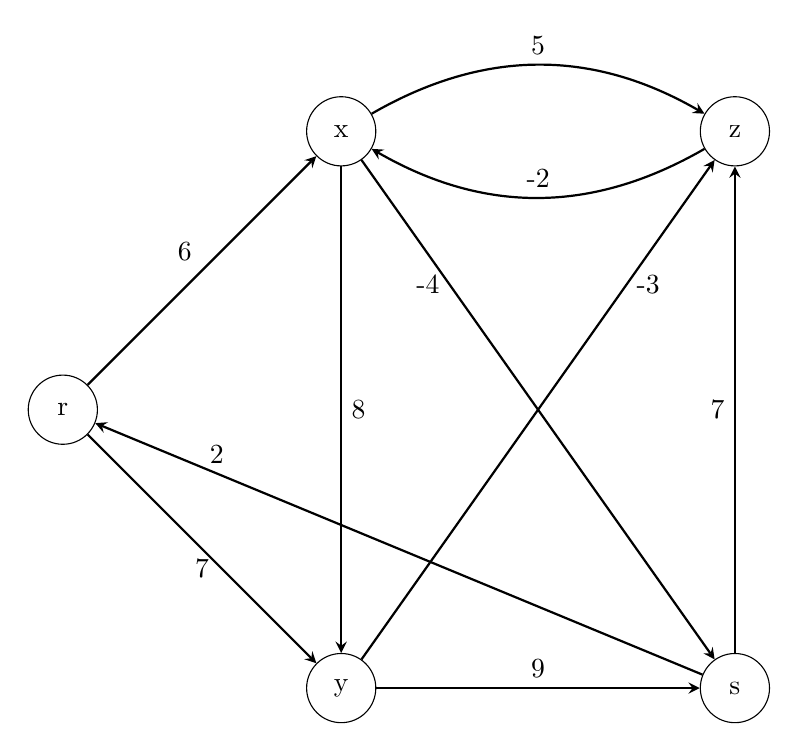
\begin{tikzpicture}[auto, baseline = 4cm, on grid, node distance = 5cm]
		\node (r) [state] {r};
		\node (x) [state, above right = of r] {x};
		\node (y) [state, below right = of r] {y};
		\node (z) [state, right = of x] {z};
		\node (s) [state, right = of y] {s};
		\path[-stealth, thick]
			(r) edge node {6} (x)
			(r) edge node [below]{7} (y)
			(s) edge node [above, pos = 0.8]{2} (r)
			(x) edge node {8} (y)
			(x) edge [bend left]node {5} (z)
			(z) edge [bend left] node [above]{-2} (x)
			(x) edge node [left, pos = 0.25]{-4} (s)
			(y) edge node [right, pos = 0.75]{-3} (z)
			(y) edge node {9} (s)
			(s) edge node {7} (z);
	\end{tikzpicture}
	Starting the algorithm we need to found the vertices reachable from $r$ (Set R) and the vertices that reach s (Set S). So we have the sets:\newline
	\begin{displaymath}
			R =\{r, 1, 2, 3, s\} \quad\text{and}\quad
			S =\{r, 1, 2, 3, s\}
	\end{displaymath}
	As $r$ belongs to the set $S$ the input doesn't pass on the test of the line 4 therefore is at least feasible.Furthermore we have that $V' = R\cap S = V$, so $D' = D$ and $n' = n$. We will start simulating the algorithm.
	\newline
	\begin{figure}[!ht]
		\centering
		\subfigure[$P(s) = \bot$]{
			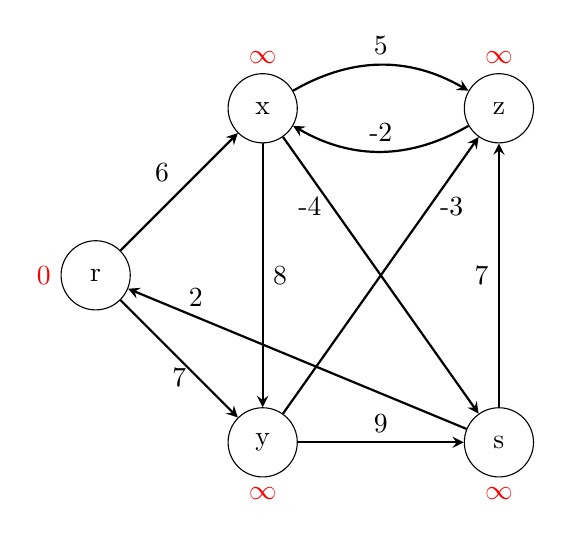
\begin{tikzpicture}[auto, baseline = 2cm, on grid, node distance = 3cm]
			\node (r) [state, label = {[red]left:0}] {r};
			\node (x) [state, above right = of r, label = {[red]above:$\infty$}] {x};
			\node (y) [state, below right = of r,label = {[red]below:$\infty$}] {y};
			\node (z) [state, right = of x,label = {[red]above:$\infty$}] {z};
			\node (s) [state, right = of y,label = {[red]below:$\infty$}] {s};
			\path[-stealth, thick]
			(r) edge node {6} (x)
			(r) edge node [below]{7} (y)
			(s) edge node [above, pos = 0.8]{2} (r)
			(x) edge node {8} (y)
			(x) edge [bend left]node {5} (z)
			(z) edge [bend left] node [above]{-2} (x)
			(x) edge node [left, pos = 0.25]{-4} (s)
			(y) edge node [right, pos = 0.75]{-3} (z)
			(y) edge node {9} (s)
			(s) edge node {7} (z);
			\end{tikzpicture}
		}
		\subfigure[$P(r) = \bot$]{
			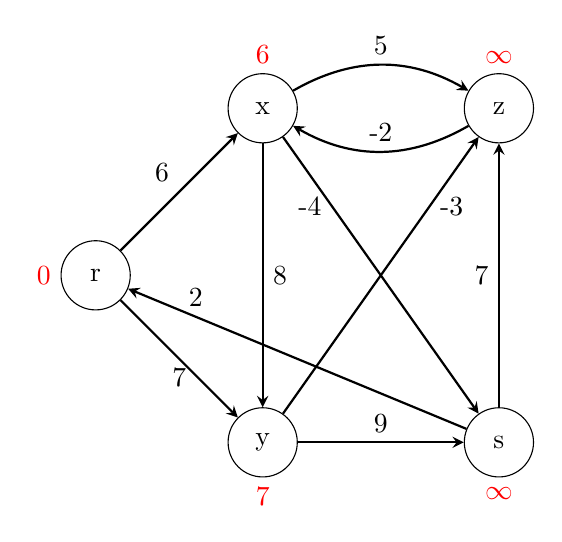
\begin{tikzpicture}[auto, baseline = 2cm, on grid, node distance = 3cm]
			\node (r) [state, label = {[red]left:0}] {r};
			\node (x) [state, above right = of r, label = {[red]above:6}] {x};
			\node (y) [state, below right = of r,label = {[red]below:7}] {y};
			\node (z) [state, right = of x,label = {[red]above:$\infty$}] {z};
			\node (s) [state, right = of y,label = {[red]below:$\infty$}] {s};
			\path[-stealth, thick]
			(r) edge node {6} (x)
			(r) edge node [below]{7} (y)
			(s) edge node [above, pos = 0.8]{2} (r)
			(x) edge node {8} (y)
			(x) edge [bend left]node {5} (z)
			(z) edge [bend left] node [above]{-2} (x)
			(x) edge node [left, pos = 0.25]{-4} (s)
			(y) edge node [right, pos = 0.75]{-3} (z)
			(y) edge node {9} (s)
			(s) edge node {7} (z);
			\end{tikzpicture}
		}
	\newline
	\subfigure[$P(r) = \left\langle r, rx, x, xs, s\right\rangle$]{
		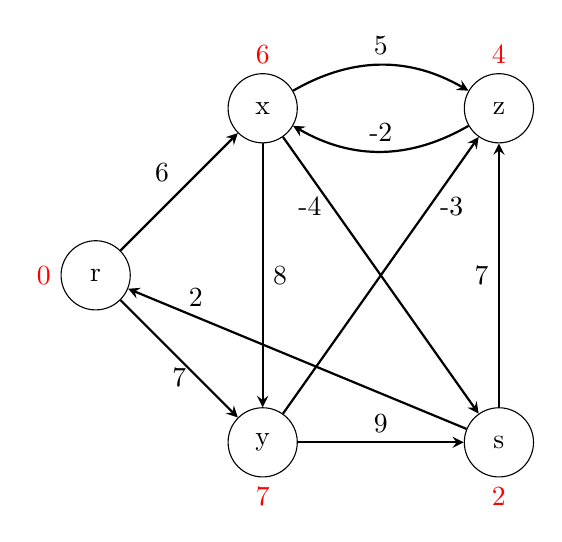
\begin{tikzpicture}[auto, baseline = 2cm, on grid, node distance = 3cm]
		\node (r) [state, label = {[red]left:0}] {r};
		\node (x) [state, above right = of r, label = {[red]above:6}] {x};
		\node (y) [state, below right = of r,label = {[red]below:7}] {y};
		\node (z) [state, right = of x,label = {[red]above:4}] {z};
		\node (s) [state, right = of y,label = {[red]below:2}] {s};
		\path[-stealth, thick]
		(r) edge node {6} (x)
		(r) edge node [below]{7} (y)
		(s) edge node [above, pos = 0.8]{2} (r)
		(x) edge node {8} (y)
		(x) edge [bend left]node {5} (z)
		(z) edge [bend left] node [above]{-2} (x)
		(x) edge node [left, pos = 0.25]{-4} (s)
		(y) edge node [right, pos = 0.75]{-3} (z)
		(y) edge node {9} (s)
		(s) edge node {7} (z);
		\end{tikzpicture}
	}
	\subfigure[$P(r) = \left\langle r, rx, x, xs, s\right\rangle$]{
		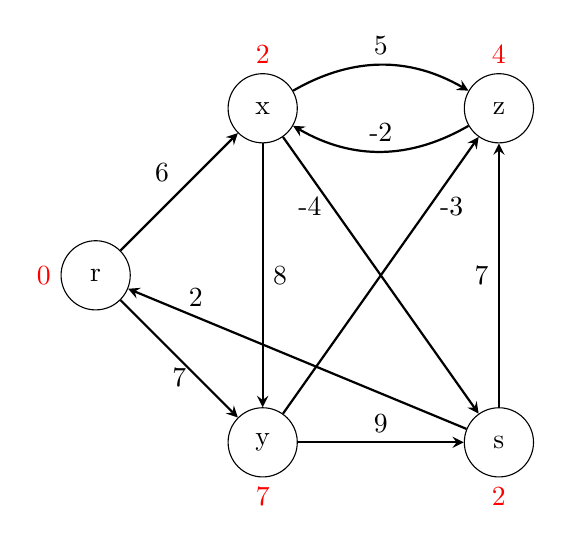
\begin{tikzpicture}[auto, baseline = 2cm, on grid, node distance = 3cm]
		\node (r) [state, label = {[red]left:0}] {r};
		\node (x) [state, above right = of r, label = {[red]above:2}] {x};
		\node (y) [state, below right = of r,label = {[red]below:7}] {y};
		\node (z) [state, right = of x,label = {[red]above:4}] {z};
		\node (s) [state, right = of y,label = {[red]below:2}] {s};
		\path[-stealth, thick]
		(r) edge node {6} (x)
		(r) edge node [below]{7} (y)
		(s) edge node [above, pos = 0.8]{2} (r)
		(x) edge node {8} (y)
		(x) edge [bend left]node {5} (z)
		(z) edge [bend left] node [above]{-2} (x)
		(x) edge node [left, pos = 0.25]{-4} (s)
		(y) edge node [right, pos = 0.75]{-3} (z)
		(y) edge node {9} (s)
		(s) edge node {7} (z);
		\end{tikzpicture}
	}
	\end{figure}
	\newpage
	\begin{figure}[!ht]
		\centering
	\subfigure[$P(r) = \left\langle r, ry, y, yz, z, zx, x, xs, s\right\rangle$]{
		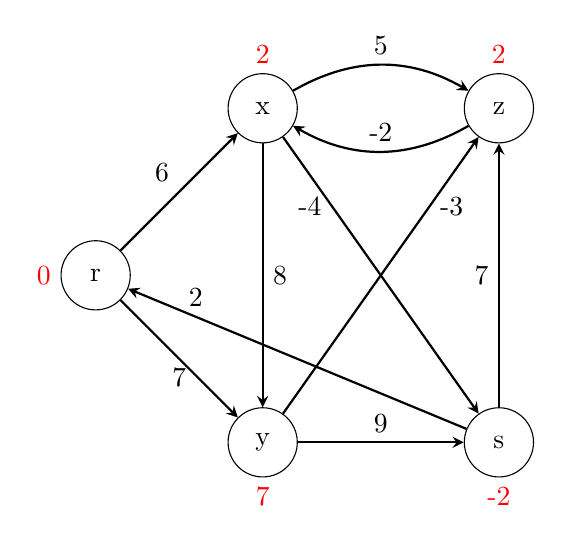
\begin{tikzpicture}[auto, baseline = 2cm, on grid, node distance = 3cm]
		\node (r) [state, label = {[red]left:0}] {r};
		\node (x) [state, above right = of r, label = {[red]above:2}] {x};
		\node (y) [state, below right = of r,label = {[red]below:7}] {y};
		\node (z) [state, right = of x,label = {[red]above:2}] {z};
		\node (s) [state, right = of y,label = {[red]below:-2}] {s};
		\path[-stealth, thick]
		(r) edge node {6} (x)
		(r) edge node [below]{7} (y)
		(s) edge node [above, pos = 0.8]{2} (r)
		(x) edge node {8} (y)
		(x) edge [bend left]node {5} (z)
		(z) edge [bend left] node [above]{-2} (x)
		(x) edge node [left, pos = 0.25]{-4} (s)
		(y) edge node [right, pos = 0.75]{-3} (z)
		(y) edge node {9} (s)
		(s) edge node {7} (z);
		\end{tikzpicture}
	}
	\end{figure}	
	We conclude that the minimum-cost walk problem given has an optimal solution which is -2 and we have a certificate ,i.e., we have a walk with cost -2 which is : $\left\langle r, ry, y, yz, z, zx, x, xs, s\right\rangle$.
	\item[\textbf{Exercise 2.}]\begin{proof} By the constraint of the optimization problem (2.1) we have that\newline $y(v) \leq y(u) + c(\alpha) \quad \text{for each } \alpha \in A\text{, where } uv := \varphi(a)$.\newline Hence $y$ is a feasible potential, by (4.1) of the Lecture notes. Since $r$ reaches $s$ the problem is feasible. By Corollary (4.5) we conclude that doesn't have any negative cycles on the digraph, so the (MinWalk) problem is bounded. Suppose Bellman-Ford Algorithm (4.1) is run on input $(D,c,r,s)$, by Theorem (5.5) exists a feasible potential in the digraph $D$ such that $c(P) = y(s) - y(r)$ where $P$ is an optimal solution for the (MinWalk) problem. By Theorem (4.2) for every $rs$-walk in $D$ we have that $c(P) \geq y(s) - y(r)$, so $c(P)$ is the maximum value that the objective function of the optimization problem (2.1) can assume, hence $y(s) - y(r)$ is the an optimal solution. Furthermore the optimization problem (2.1) has the same optimal value of the (MinWalk) problem.
	\end{proof}
	\item[\textbf{Exercise 6.}] 
	\item[\textbf{Exercise 9.}] ($\Rightarrow$)
	\begin{proof}
		If $\varphi$ is a homomorphism, we have that for each $\mu \in \mathbb{R}$, one has $\varphi~(L_{\mathcal{O}}(\mu))~\subseteq~L_{\mathcal{P}}(\mu)$. 
		Suppose that $\exists x \in X$ such that $\alpha g(\varphi(x)) < \alpha f(x)$, so set $\mu = f(x)$, we have that $x \in L_{\mathcal{O}}(\mu)$, because $\alpha f(x) \geq \alpha \mu = \alpha f(x)$, so $\varphi(x) \in \varphi~(L_{\mathcal{O}}(\mu))$, but $\varphi (x) \notin L_{\mathcal{P}}(\mu)$, since $\alpha g(\varphi(x)) < \alpha f(x) = \alpha \mu$, however this contradicts the fact that $\varphi$ is a homomorphism. Thus, $\alpha g(\varphi(x)) \geq \alpha f(x)$.
	\end{proof} 
	($\Leftarrow$)
	\begin{proof}
		If for each $x \in X$, one has $\alpha g(\varphi (x)) \geq \alpha f(x)$. Let $x \in X$, and let $\mu \in \mathbb{R}$ such that $x \in L_{\mathcal{O}}(\mu)$ (Note that $\varphi (x) \in \varphi(L_{\mathcal{O}}(\mu))$), i.e., $\alpha f(x) \geq \alpha \mu$. Since $\alpha g(\varphi (x)) \geq \alpha f(x)$, we have that $\alpha g(\varphi (x)) \geq \alpha f(x) \geq \alpha \mu \Rightarrow \alpha g(\varphi (x)) \geq \alpha \mu$. Hence, $\varphi(x) \in L_{\mathcal{P}}(\mu)$. We proved that if a element belongs to the set $\varphi(L_{\mathcal{O}}(\mu))$ so this element belongs to $L_{\mathcal{P}}(\mu)$ too, i.e., $\varphi~(L_{\mathcal{O}}(\mu))~\subseteq~L_{\mathcal{P}}(\mu)$ that is $\varphi$ is a homomorphism.
	\end{proof}
	\item[\textbf{Exercise 12.}]
\end{enumerate}

\end{document}
